% Drawing 85/05-6 -- folder 85, batch 05, archive page 92 (PDF page 93).
% Transcription: en bas à droite, un petit segment horizontal, son extrémité gauche marquée d'un point, avec « $-1$ » et « $1$ » sous ses extrémités
% Kind: segment from -1 to 1. Method 2 (schematic redraw from the facsimile). Status: ok.
% Notes: Ink. A short heavy segment with a dot at its left end; -1 and 1 below its ends. Redrawn 2026-11-12 (issue 128): to check again.
% Coordinates: 1 unit = 1 mm = 1/100 of the crop width (bbox in page fractions: [0.62, 0.7, 0.92, 0.76]).
% Redrawn by Claude (claude-fable-5-2), issue #128, 2026-11-12; not checked by a human; not compiled (no TeX in the session).
% Rights: reproduces part of the work -- behind RENDER_TRANSCRIPTS, never published by itself.
\documentclass[tikz,border=3pt]{standalone}
\usepackage{amsmath,amssymb}
\usetikzlibrary{patterns,arrows.meta}
\tikzset{pencil/.style={black!45}, struck/.style={black!35}, mpt/.style={circle,draw,inner sep=1.3pt}, pt/.style={circle,fill,inner sep=0.9pt}, opt/.style={circle,draw,fill=white,inner sep=1.1pt}}
\begin{document}
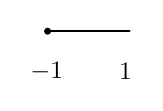
\begin{tikzpicture}[x=1mm,y=1mm,line cap=round,line join=round,font=\scriptsize]
\draw[thick] (42.6,-11.3) -- (53,-11.3);
\node[pt] at (42.6,-11.3) {};
\node[inner sep=1pt] at (42.5,-16.4) {\small $-1$};
\node[inner sep=1pt] at (52.5,-16.4) {\small $1$};
\end{tikzpicture}
\end{document}
